\documentclass{beamer}
\usepackage[utf8]{inputenc}

\usetheme{Madrid}
\usecolortheme{default}
\usepackage{amsmath,amssymb,amsfonts,amsthm}
\usepackage{txfonts}
\usepackage{tkz-euclide}
\usepackage{listings}
\usepackage{adjustbox}
\usepackage{array}
\usepackage{tabularx}
\usepackage{gvv}
\usepackage{lmodern}
\usepackage{circuitikz}
\usepackage{tikz}
\usepackage{graphicx}

\setbeamertemplate{page number in head/foot}[totalframenumber]

\usepackage{tcolorbox}
\tcbuselibrary{minted,breakable,xparse,skins}



\definecolor{bg}{gray}{0.95}
\DeclareTCBListing{mintedbox}{O{}m!O{}}{%
  breakable=true,
  listing engine=minted,
  listing only,
  minted language=#2,
  minted style=default,
  minted options={%
    linenos,
    gobble=0,
    breaklines=true,
    breakafter=,,
    fontsize=\small,
    numbersep=8pt,
    #1},
  boxsep=0pt,
  left skip=0pt,
  right skip=0pt,
  left=25pt,
  right=0pt,
  top=3pt,
  bottom=3pt,
  arc=5pt,
  leftrule=0pt,
  rightrule=0pt,
  bottomrule=2pt,
  toprule=2pt,
  colback=bg,
  colframe=orange!70,
  enhanced,
  overlay={%
    \begin{tcbclipinterior}
    \fill[orange!20!white] (frame.south west) rectangle ([xshift=20pt]frame.north west);
    \end{tcbclipinterior}},
  #3,
}
\lstset{
    language=C,
    basicstyle=\ttfamily\small,
    keywordstyle=\color{blue},
    stringstyle=\color{orange},
    commentstyle=\color{green!60!black},
    numbers=left,
    numberstyle=\tiny\color{gray},
    breaklines=true,
    showstringspaces=false,
}
%------------------------------------------------------------
%This block of code defines the information to appear in the
%Title page
\title %optional
{1.2.26}
\date{August 28,2025}
%\subtitle{A short story}

\author % (optional)
{Hemanth Reddy-AI25BTECH11018}



\begin{document}


\frame{\titlepage}
\begin{frame}{Question}
Rain is falling vertically with a speed of $35~ms^{-1}$. A woman rides a bicycle with a speed of $12~ms^{-1}$ in east to west direction. What is the direction in which she should hold her umbrella~?
\end{frame}



\begin{frame}{Theoretical Solution}
\textbf{Solution:}\\
Velocity of rain $\overrightarrow{v}_{rain}=\myvec{0\\
-35}$\\
Velocity of woman $\overrightarrow{v}_{woman}=\myvec{-12\\0}$\\
The relative velocity of rain with respect to the woman is:$\overrightarrow{v}_{rel}=\overrightarrow{v}_{rain}-\overrightarrow{v}_{woman}\\ = \myvec{0\\
-35}-\myvec{-12\\0}= \myvec{12\\-35}$\\
Let $\overrightarrow{a} = \myvec{1\\0}$\\

\end{frame}

\begin{frame}{Theoretical Solution}

Let $\theta$ be the angle with horizontal\\
$\cos \theta= \frac{a^{T} v_{rel}}{||a||v_{rel}||}$

$\cos \theta= \frac{12}{37}$
\end{frame}




\begin{frame}[fragile]
    \frametitle{C Code }
    \begin{lstlisting}

#include <stdio.h>
#include <math.h>

int main() {
    // Components of the relative velocity vector
    double vx = 12.0;      // horizontal component
    double vy = -35.0;     // vertical component

    // Calculate magnitude of relative velocity vector
    double magnitude = sqrt(vx * vx + vy * vy);

    // Calculate cos(theta)
    double cos_theta = vx / magnitude;

    // Output result
    printf("cos(theta) = %.5f\n", cos_theta);
    
    return 0;
}

    \end{lstlisting}
\end{frame}




\begin{frame}[fragile]
    \frametitle{Python Code}
    \begin{lstlisting}

import matplotlib.pyplot as plt
from mpl_toolkits.mplot3d import Axes3D
import numpy as np

# Define vector components
rain_velocity = np.array([0, 0, -35])    # Rain falling vertically
woman_velocity = np.array([-12, 0, 0])   # Woman moving east to west
relative_velocity = rain_velocity - woman_velocity  # Relative velocity of rain w.r.t woman

# Origin point for vectors
origin = np.array([0, 0, 0])

# Plot setup
fig = plt.figure(figsize=(10, 8))
ax = fig.add_subplot(111, projection='3d')

# Plot rain velocity vector (blue)
ax.quiver(*origin, *rain_velocity, color='blue', label='Rain Velocity', arrow_length_ratio=0.1)

# Plot woman velocity vector (green)
ax.quiver(*origin, *woman_velocity, color='green', label='Woman Velocity', arrow_length_ratio=0.1)

# Plot relative velocity vector (red)
ax.quiver(*origin, *relative_velocity, color='red', label='Relative Velocity (Umbrella Direction)', arrow_length_ratio=0.1)

# Set axis labels
ax.set_xlabel('X (East-West)')
ax.set_ylabel('Y (North-South)')
ax.set_zlabel('Z (Vertical)')

# Set plot limits
ax.set_xlim([-20, 20])
ax.set_ylim([-20, 20])
ax.set_zlim([-40, 10])

# Title and legend
ax.set_title('Direction to Hold Umbrella (Relative Velocity)')
ax.legend()

# Save the figure as an image
plt.savefig("fig.png", dpi=300)
# Show the plot
plt.show()


    \end{lstlisting}
\end{frame}







\begin{frame}[fragile]
    \frametitle{Python Code}
    \begin{lstlisting}

# Plot rain velocity vector (blue)
ax.quiver(*origin, *rain_velocity, color='blue', label='Rain Velocity', arrow_length_ratio=0.1)

# Plot woman velocity vector (green)
ax.quiver(*origin, *woman_velocity, color='green', label='Woman Velocity', arrow_length_ratio=0.1)

# Plot relative velocity vector (red)
ax.quiver(*origin, *relative_velocity, color='red', label='Relative Velocity (Umbrella Direction)', arrow_length_ratio=0.1)

# Set axis labels
ax.set_xlabel('X (East-West)')
ax.set_ylabel('Y (North-South)')
ax.set_zlabel('Z (Vertical)')

    \end{lstlisting}
\end{frame}


\begin{frame}[fragile]
    \frametitle{Python Code}
    \begin{lstlisting}

# Set plot limits
ax.set_xlim([-20, 20])
ax.set_ylim([-20, 20])
ax.set_zlim([-40, 10])

# Title and legend
ax.set_title('Direction to Hold Umbrella (Relative Velocity)')
ax.legend()

# Save the figure as an image
plt.savefig("fig.png", dpi=300)
# Show the plot
plt.show()

    \end{lstlisting}
\end{frame}




  
\begin{frame}{Plot}
\begin{figure}
    \centering
    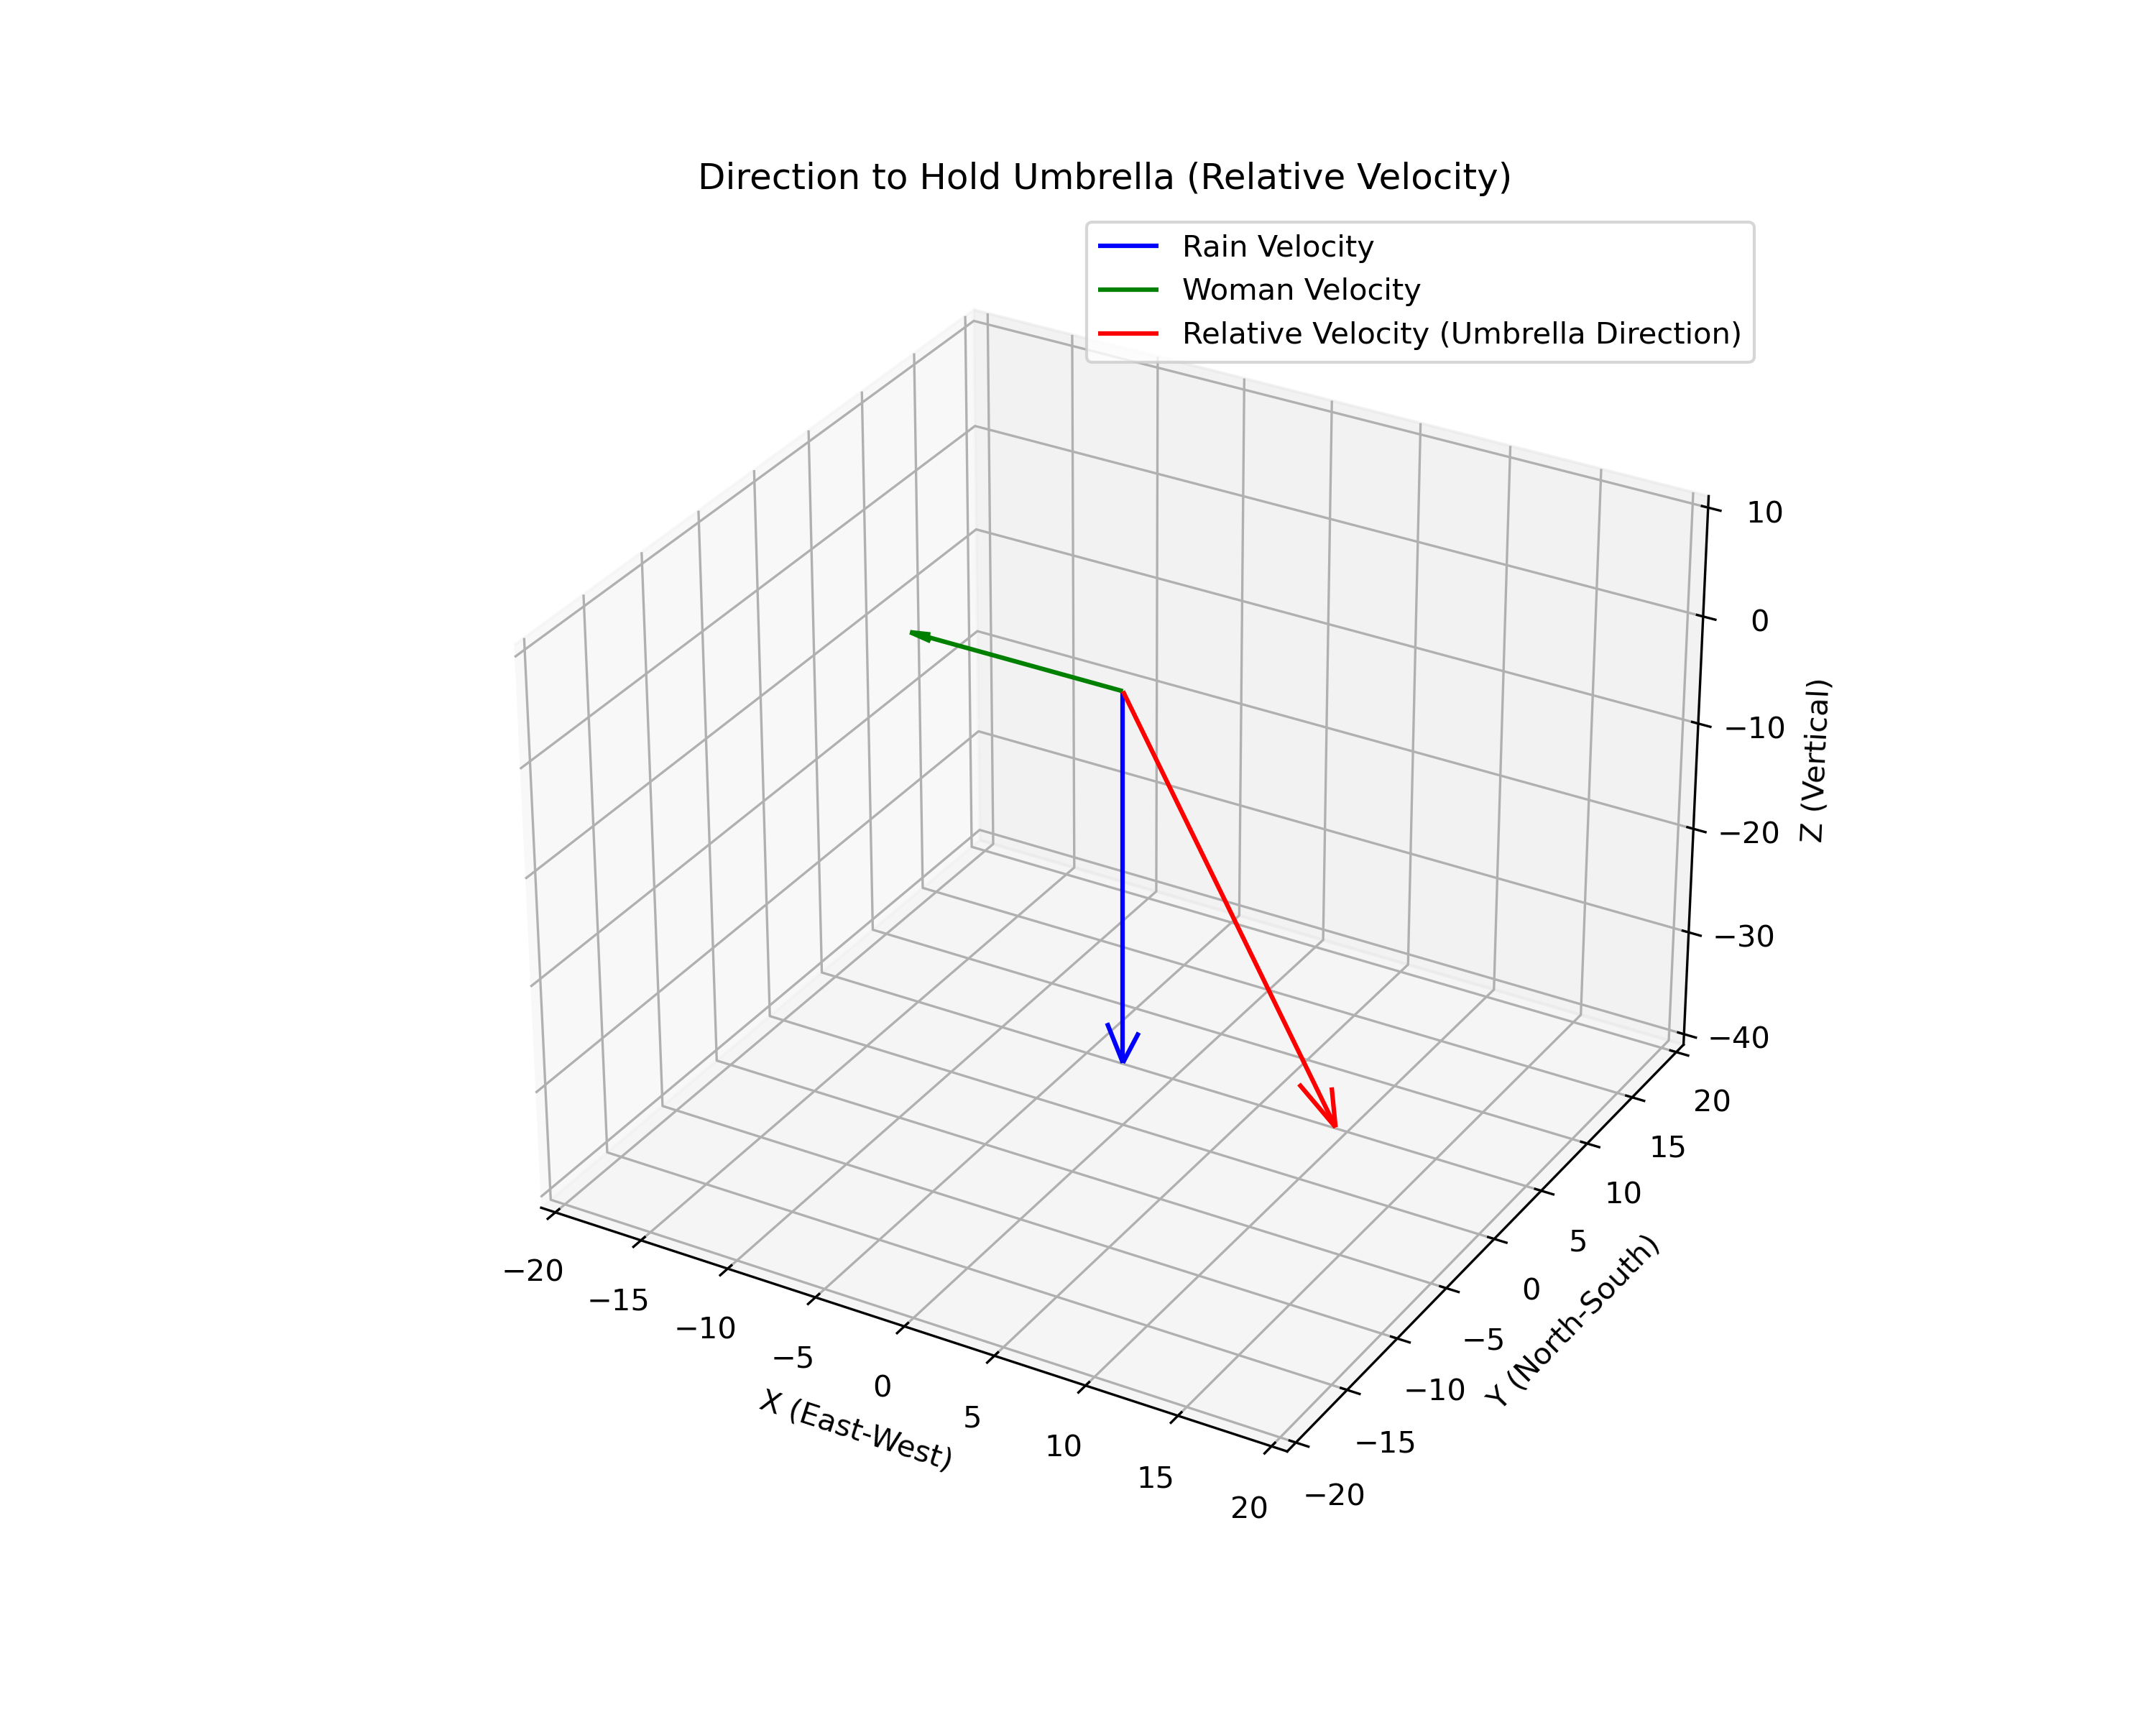
\includegraphics[width=0.8\columnwidth]{figs/fig.png}
    \caption{}
    \label{fig:figs/fig.png}
\end{figure}
\end{frame}




\end{document}
